\documentclass[11pt]{article}

% ----- lightweight preamble -----
\usepackage[a4paper,margin=1.8cm]{geometry}
\usepackage{amsmath,amssymb}
\usepackage{tikz}
\usepackage{tikz-cd}
\usetikzlibrary{arrows.meta,positioning,calc,fit,backgrounds,
  shapes.geometric,chains,decorations.pathreplacing}
\usepackage[most]{tcolorbox}
\usepackage{parskip}
\usepackage{xcolor}

\definecolor{gold}{RGB}{200,140,0}
\definecolor{kas}{RGB}{30,110,190}
\definecolor{ink}{RGB}{40,40,40}
\definecolor{soft}{RGB}{245,245,248}
\definecolor{grn}{RGB}{30,140,80}
\definecolor{pur}{RGB}{130,70,170}
\definecolor{red2}{RGB}{200,50,50}

\newtcolorbox{note}[1][]{colback=soft,colframe=ink,boxrule=0.4pt,
  arc=2pt,left=6pt,right=6pt,top=4pt,bottom=4pt,#1}

% "one gadget" badge colours: the three faces of the pattern
\definecolor{faceL}{RGB}{30,140,80}   % linearized trace L_k
\definecolor{faceF}{RGB}{200,140,0}   % Frobenius / doubling
\definecolor{faceC}{RGB}{130,70,170}  % cyclotomic coset bookkeeping

\tikzset{
  obj/.style={draw=ink,rounded corners=3pt,fill=soft,inner sep=5pt,font=\small,align=center},
  thm/.style={draw=ink,rounded corners=3pt,fill=white,inner sep=4pt,
    font=\small,align=center,minimum height=8mm},
  gnode/.style={circle,draw=gold,fill=gold!12,minimum size=7mm,font=\small,inner sep=0pt},
  knode/.style={circle,draw=kas,fill=kas!12,minimum size=7mm,font=\small,inner sep=0pt},
  arr/.style={-{Stealth[length=2.5mm]},thick},
  dep/.style={-{Stealth[length=2.2mm]},thick,ink},
  badge/.style={circle,inner sep=0pt,minimum size=3.6mm,font=\scriptsize\bfseries,text=white},
}
\newcommand{\bL}{\tikz[baseline=-0.6ex]\node[badge,fill=faceL]{L};}
\newcommand{\bF}{\tikz[baseline=-0.6ex]\node[badge,fill=faceF]{F};}
\newcommand{\bC}{\tikz[baseline=-0.6ex]\node[badge,fill=faceC]{C};}

\title{\vspace{-1.5cm}\textbf{Dobbertin (1999): one gadget, many theorems}\\[2pt]
\large A picture book of Kasami power functions, permutation polynomials
and cyclic difference sets}
\author{\small Visual summary --- \texttt{Dobbertin1999MVP} (Lean\,/\,Mathlib)}
\date{}

\begin{document}
\maketitle
\vspace{-1.1cm}

\begin{note}
\textbf{Thesis.} Every result of the paper is the \emph{same small gadget}
seen from a new angle. The gadget has three faces:
\bL~the \textbf{linearized trace} $L_k(x)=\sum_{i<k}x^{2^i}$ (a truncated,
additive polynomial);
\bF~\textbf{Frobenius} $x\mapsto x^2$ (``freshman's dream'', doubling on
exponents);
\bC~\textbf{cyclotomic-coset} bookkeeping (orbits of doubling mod $2^n{-}1$).
The permutation criterion, APN, the MCM bridge, the explicit inverse, and
the difference sets are all this one gadget, propagated. Boxes marked
\checkmark\ are machine-checked in Lean.
\end{note}

%======================================================================
\section*{0. The gadget}

\begin{center}
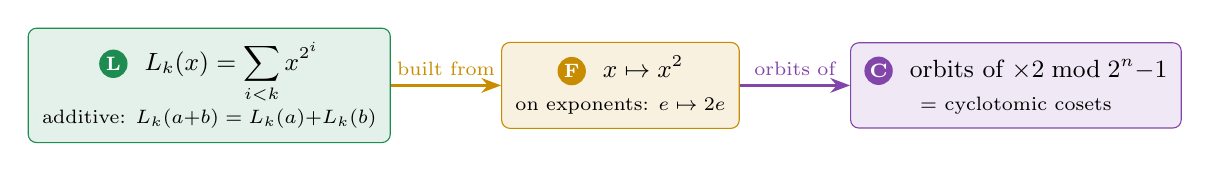
\begin{tikzpicture}[node distance=6mm]
  \node[obj,fill=faceL!12,draw=faceL] (L)
    {\bL\ \ $L_k(x)=\displaystyle\sum_{i<k}x^{2^i}$\\[1pt]
     \scriptsize additive: $L_k(a{+}b)=L_k(a){+}L_k(b)$};
  \node[obj,fill=faceF!12,draw=faceF,right=14mm of L] (F)
    {\bF\ \ $x\mapsto x^{2}$\\[1pt]
     \scriptsize on exponents: $e\mapsto 2e$};
  \node[obj,fill=faceC!12,draw=faceC,right=14mm of F] (C)
    {\bC\ \ orbits of $\times2\bmod 2^n{-}1$\\[1pt]
     \scriptsize $=$ cyclotomic cosets};
  \draw[arr,faceF] (L) -- node[above,font=\scriptsize]{built from} (F);
  \draw[arr,faceC] (F) -- node[above,font=\scriptsize]{orbits of} (C);
\end{tikzpicture}
\end{center}

\begin{center}\small
Telescoping identity that glues \bL\ to \bF:\quad
$L_k(x^2+x)=x^{2^k}+x$\qquad
{\scriptsize(\texttt{truncTrace\_artin\_schreier}, generalised in
\texttt{Pearl.lean})}\ \checkmark
\end{center}

%======================================================================
\section*{1. The whole paper on one page (dependency map)}

Arrows $=$ ``used to prove''. Each node carries the faces of the gadget it
leans on.

\begin{center}
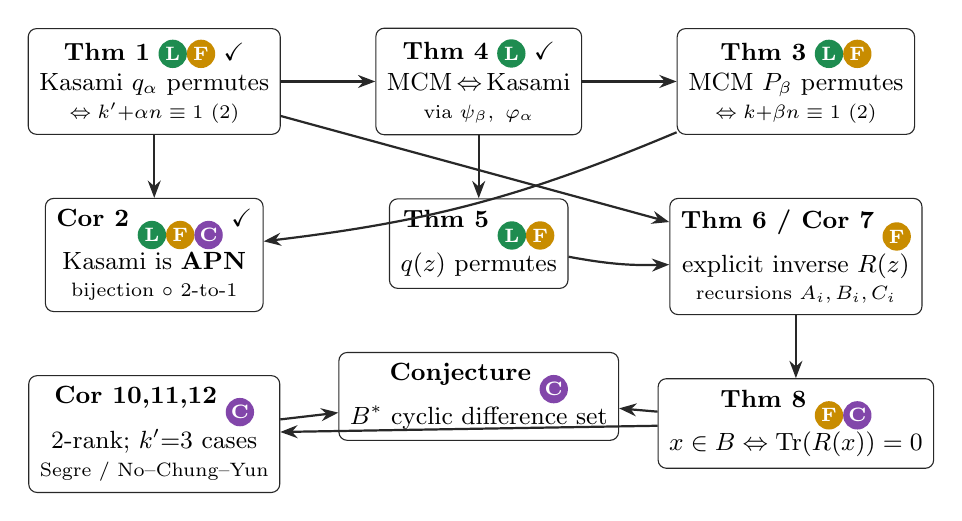
\begin{tikzpicture}[node distance=8mm and 12mm]
  % row 1
  \node[thm] (t1) {\textbf{Thm 1} \bL\bF\ \checkmark\\
    Kasami $q_\alpha$ permutes\\[-1pt]
    \scriptsize$\Leftrightarrow k'{+}\alpha n\equiv1\ (2)$};
  \node[thm,right=of t1] (t4) {\textbf{Thm 4} \bL\ \checkmark\\
    MCM\,$\Leftrightarrow$\,Kasami\\[-1pt]
    \scriptsize via $\psi_\beta,\ \varphi_\alpha$};
  \node[thm,right=of t4] (t3) {\textbf{Thm 3} \bL\bF\\
    MCM $P_\beta$ permutes\\[-1pt]
    \scriptsize$\Leftrightarrow k{+}\beta n\equiv1\ (2)$};
  % row 2
  \node[thm,below=of t1] (c2) {\textbf{Cor 2} \bL\bF\bC\ \checkmark\\
    Kasami is \textbf{APN}\\[-1pt]
    \scriptsize bijection $\circ$ 2-to-1};
  \node[thm,below=of t4] (t5) {\textbf{Thm 5} \bL\bF\\
    $q(z)$ permutes};
  \node[thm,below=of t3] (t6) {\textbf{Thm 6 / Cor 7} \bF\\
    explicit inverse $R(z)$\\[-1pt]
    \scriptsize recursions $A_i,B_i,C_i$};
  % row 3
  \node[thm,below=of t6] (t8) {\textbf{Thm 8} \bF\bC\\
    $x\in B\Leftrightarrow \mathrm{Tr}(R(x))=0$};
  \node[thm,below=of c2] (dc) {\textbf{Cor 10,11,12} \bC\\
    $2$-rank; $k'{=}3$ cases\\[-1pt]
    \scriptsize Segre / No--Chung--Yun};
  \node[thm,below=of t5] (cj) {\textbf{Conjecture} \bC\\
    $B^\ast$ cyclic difference set};

  % edges
  \draw[dep] (t1) -- (t4);
  \draw[dep] (t4) -- (t3);
  \draw[dep] (t1) -- (c2);
  \draw[dep] (t3) to[bend left=8] (c2);
  \draw[dep] (t4) -- (t5);
  \draw[dep] (t1) -- (t6);
  \draw[dep] (t5) to[bend right=6] (t6);
  \draw[dep] (t6) -- (t8);
  \draw[dep] (t8) -- (dc);
  \draw[dep] (t8) -- (cj);
  \draw[dep] (dc) -- (cj);
\end{tikzpicture}
\end{center}

\begin{center}\small
\bL\ linearized trace \quad \bF\ Frobenius \quad \bC\ cyclotomic cosets
\qquad \checkmark\ formalised in Lean
\end{center}

%======================================================================
\section*{2. Permutation criterion (Thm 1 $=$ Thm 3): a parity square}

Both criteria have the \emph{same shape}: ``$q_\alpha$ (resp. $P_\beta$)
permutes $\iff$ a single parity is odd''. The operator on the left of the
linearized equation is the gadget \bL.

\begin{center}
\begin{tikzcd}[column sep=large,row sep=large]
\text{Kasami } q_\alpha \arrow[r,"\text{Thm 4: }\psi_\beta/\varphi_\alpha"]
  \arrow[d,"\text{permutes?}"'] &
\text{MCM } P_\beta \arrow[d,"\text{permutes?}"] \\
k'+\alpha n\equiv1\ (2) \arrow[r,leftrightarrow,"\text{same parity}"'] &
k+\beta n\equiv1\ (2)
\end{tikzcd}
\end{center}

%======================================================================
\section*{3. Theorem 4: the bridge is an isomorphism of self-maps}

$\psi_\beta(x)=\sum_{i<k}x^{2^i}+\beta\,\mathrm{Tr}(x)$ (that is \bL, plus a
trace) is a \emph{bijective intertwiner}: it conjugates the Kasami power map
into the MCM power map. In the category \texttt{Endo} of sets-with-a-self-map
this is one iso.

\begin{center}
\begin{tikzcd}[column sep=huge,row sep=large]
L \arrow[r,shift left=1.1ex,"\psi_\beta"]
  \arrow[d,"q_\alpha"'] &
L \arrow[l,shift left=1.1ex,"\varphi_\alpha"]
  \arrow[d,"P_\beta"] \\
L \arrow[r,shift left=1.1ex,"\psi_\beta"] &
L \arrow[l,shift left=1.1ex,"\varphi_\alpha"]
\end{tikzcd}
\qquad
$P_\beta=\psi_\beta\circ q_\alpha\circ\psi_\beta^{-1}$
\end{center}

\begin{center}\small
Lean: \texttt{mcm\_permutation}, \texttt{mcm\_permutation\_ktransfer}
(\checkmark); category home \texttt{Endo}/\texttt{isoOfEquiv}
(\texttt{ShiftConjugacy.lean}, \checkmark).
\end{center}

%======================================================================
\section*{4. Corollary 2: APN $=$ (bijection) $\circ$ (two-to-one)}

The Kasami derivative factors through the gadget. The right factor is the
\emph{Artin--Schreier} map $t\mapsto t^{2^k}+t=L_k(t^2+t)$ --- exactly
two-to-one because $\gcd(k,n)=1$ (\bC). Bijection $\circ$ 2-to-1
$\Rightarrow$ every fibre has $0$ or $2$ points $\Rightarrow$ APN.

\begin{center}
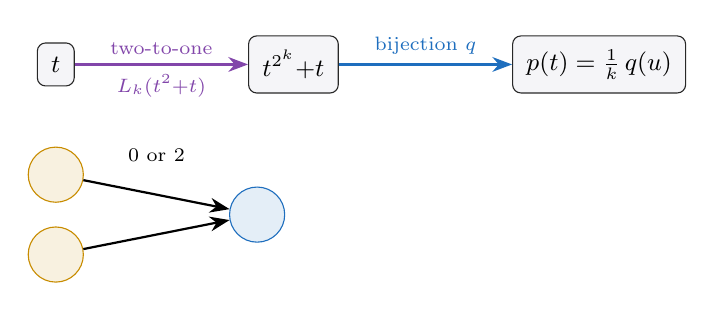
\begin{tikzpicture}[node distance=16mm]
  \node[obj] (t) {$t$};
  \node[obj,right=22mm of t] (u) {$t^{2^k}{+}t$};
  \node[obj,right=22mm of u] (p) {$p(t)=\tfrac1k\,q(u)$};
  \draw[arr,faceC] (t) -- node[above,font=\scriptsize,faceC]{two-to-one}
     node[below,font=\scriptsize]{$L_k(t^2{+}t)$} (u);
  \draw[arr,kas] (u) -- node[above,font=\scriptsize,kas]{bijection $q$} (p);
  % fibre picture
  \begin{scope}[yshift=-14mm]
    \node[gnode] (a){}; \node[gnode,below=3mm of a] (b){};
    \node[knode,right=22mm of $(a)!0.5!(b)$] (c){};
    \draw[arr] (a)--(c); \draw[arr] (b)--(c);
    \node[font=\scriptsize] at ($(a)!0.5!(c)+(0,0.5)$){$0$ or $2$};
  \end{scope}
\end{tikzpicture}
\end{center}

\begin{center}\small
Key identity (the concrete Gold\,$\leftrightarrow$\,Kasami bridge, \checkmark):\quad
$\big((x{+}1)^d+x^d+1\big)\,(x^2{+}x)^{2^k}=(x^{2^k}{+}x)^{2^k+1}$\\[1pt]
Lean: \texttt{kasami\_key\_identity}, \texttt{gold\_permutation},
\texttt{kasami\_is\_apn}, \texttt{kasami\_is\_apn\_solution\_count}.
\end{center}

%======================================================================
\section*{5. Theorem 6 / Cor 7: the same shift, iterated $\Rightarrow$ inverse}

Feeding the linearized equation through Frobenius \bF\ repeatedly spawns one
relation per level $i$ (eq.~(10)); the three families $A_i,B_i,C_i$ obey
\emph{one} two-step recursion. Their $2\times2$ Wronskian cross-invariants
(eqs.~(11)--(13)) are conserved, which collapses the would-be cubic to a
line: the unique root is the explicit inverse $R$.

\begin{center}
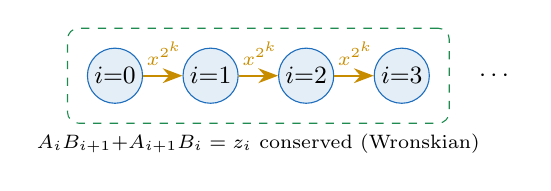
\begin{tikzpicture}[start chain=going right,node distance=5mm]
  \foreach \i in {0,1,2,3} {
    \node[on chain,knode] (r\i) {$i{=}\i$};
  }
  \node[on chain,font=\small] {$\cdots$};
  \foreach \i/\j in {0/1,1/2,2/3} {
    \draw[arr,faceF] (r\i) -- node[above,font=\scriptsize]{$x^{2^k}\!$} (r\j);
  }
  % invariant under the ladder
  \begin{scope}[on background layer]
    \node[draw=grn,dashed,rounded corners,fit=(r0)(r3),inner sep=7pt,
      label=below:{\scriptsize $A_iB_{i+1}{+}A_{i+1}B_i=z_i$ conserved (Wronskian)}]{};
  \end{scope}
\end{tikzpicture}
\end{center}

\begin{center}
\begin{tikzcd}[column sep=large]
\text{cubic } x^3{+}A_2x^2{+}A_1x{+}A_0
  \arrow[r,"A_1=A_0=0"] &
\text{line } x=R(y)
  \arrow[r,"q^{-1}(1/y)=R(y)"] &
\text{explicit inverse}
\end{tikzcd}
\end{center}

\begin{center}\small
Conserved cross-invariant formalised: \texttt{Theorem6.cross\_invariant},
\texttt{Theorem6.key\_identity} (\checkmark, char.\ 2 cancellation).
\end{center}

%======================================================================
\section*{6. Theorem 8 $+$ Conjecture: the coset combinatorics of $B$}

$R$ from Thm 6 defines the set $B=\{x:\mathrm{Tr}(R(x))=0\}$ (Thm 8, a trace
test \bF). The Section-4 conjecture is pure \bC: $B^\ast$ is a difference set
in the cyclic group $L^\ast$, and the $k\leftrightarrow n{-}k$ /
$(k,k')\leftrightarrow(n{-}k,n{-}k')$ symmetries are cyclotomic shifts.

\begin{center}
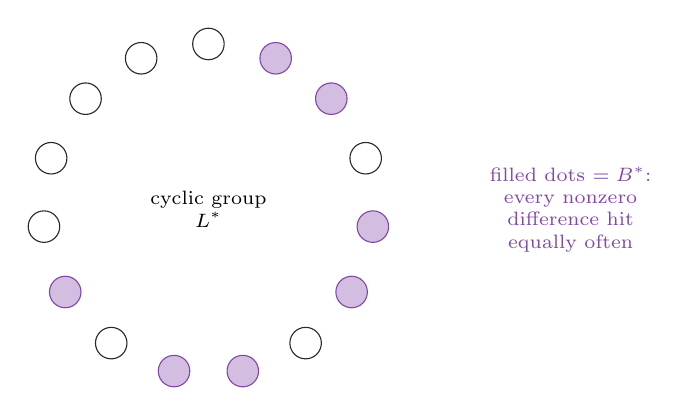
\begin{tikzpicture}
  % cyclic group as a ring of dots, some in B (filled)
  \def\N{15}
  \foreach \i in {0,...,14} {
    \pgfmathsetmacro\ang{90-\i*360/\N}
    \pgfmathtruncatemacro\inB{ (\i==1)||(\i==2)||(\i==4)||(\i==8)||(\i==5)||(\i==10)||(\i==7) ? 1 : 0 }
    \ifnum\inB=1
      \node[circle,draw=pur,fill=pur!35,minimum size=4mm,inner sep=0pt]
        (n\i) at (\ang:2.1){};
    \else
      \node[circle,draw=ink,fill=white,minimum size=4mm,inner sep=0pt]
        (n\i) at (\ang:2.1){};
    \fi
  }
  \node[font=\scriptsize,align=center] at (0,0)
    {cyclic group\\ $L^\ast$};
  \node[pur,font=\scriptsize,align=center] at (4.6,0)
    {filled dots $=B^\ast$:\\ every nonzero\\ difference hit\\ equally often};
\end{tikzpicture}
\end{center}

\begin{center}\small
Conjecture (up to cyclotomic equivalence): only $d=2^k{+}1$ (Gold) and
$d=2^{2k}{-}2^k{+}1$ (Kasami) yield this $B$; contains Segre / Maschietti
(1998) and No--Chung--Yun (1998) / Dillon $k'{=}3$ cases.
\end{center}

%======================================================================
\section*{7. Why it is ``one pattern'': the census as a table}

\begin{center}\small
\renewcommand{\arraystretch}{1.25}
\begin{tabular}{@{}l l l@{}}
\textbf{Result} & \textbf{Gadget face used} & \textbf{Lean} \\ \hline
Thm 1 --- Kasami permutation criterion & \bL\ operator, \bF\ shift &
  \texttt{mcm\_permutation\_ktransfer}\ \checkmark\\
Cor 2 --- Kasami APN & \bL$\circ$\bF\ telescope, \bC\ 2-to-1 &
  \texttt{kasami\_is\_apn}\ \checkmark\\
Thm 3 --- MCM permutation criterion & \bL\ operator (dual) & via Thm 4\\
Thm 4 --- MCM\,$\Leftrightarrow$\,Kasami ($\psi_\beta$) & \bL\ $=$ intertwiner &
  \texttt{mcm\_permutation}\ \checkmark\\
Thm 5 --- $q$ is a permutation & \bL, \bF & (implied)\\
Thm 6 / Cor 7 --- explicit inverse $R$ & \bF\ iterated, Wronskian &
  \texttt{Theorem6.*}\ \checkmark\\
Thm 8 --- difference set $B$ & \bF\ trace test, \bC & ---\\
Cor 10/11/12 --- $2$-rank, $k'{=}3$ & \bC\ coset counting & ---\\
Conjecture --- $B^\ast$ difference set & \bC\ cyclotomic equivalence & ---\\
\end{tabular}
\end{center}

\begin{note}
\textbf{One sentence.} The linearized trace \bL\ and Frobenius \bF\ give the
permutation criterion; telescoping \bL$\circ$\bF\ plus a two-to-one
Artin--Schreier map (\bC) gives APN; the bijective intertwiner \bL\ gives the
MCM bridge; iterating \bF\ with conserved Wronskians gives the inverse; and
coset bookkeeping \bC\ carries it all into the difference sets --- one gadget,
propagated from the smallest identity to the global conjecture.
\end{note}

%======================================================================
\section*{8. Formal status (what is machine-checked)}

\begin{center}
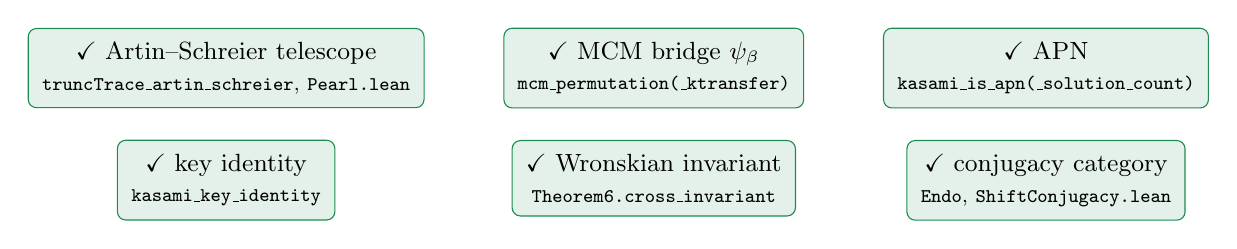
\begin{tikzpicture}[node distance=4mm and 10mm]
  \node[obj,fill=grn!12,draw=grn] (a){\checkmark\ Artin--Schreier telescope\\
    \scriptsize\texttt{truncTrace\_artin\_schreier}, \texttt{Pearl.lean}};
  \node[obj,fill=grn!12,draw=grn,right=of a] (b){\checkmark\ MCM bridge $\psi_\beta$\\
    \scriptsize\texttt{mcm\_permutation(\_ktransfer)}};
  \node[obj,fill=grn!12,draw=grn,right=of b] (c){\checkmark\ APN\\
    \scriptsize\texttt{kasami\_is\_apn(\_solution\_count)}};
  \node[obj,fill=grn!12,draw=grn,below=of a] (d){\checkmark\ key identity\\
    \scriptsize\texttt{kasami\_key\_identity}};
  \node[obj,fill=grn!12,draw=grn,below=of b] (e){\checkmark\ Wronskian invariant\\
    \scriptsize\texttt{Theorem6.cross\_invariant}};
  \node[obj,fill=grn!12,draw=grn,below=of c] (f){\checkmark\ conjugacy category\\
    \scriptsize\texttt{Endo}, \texttt{ShiftConjugacy.lean}};
\end{tikzpicture}
\end{center}

\vfill
\begin{center}\scriptsize
Checked \texttt{sorry}-free in Lean\,/\,Mathlib. Sources: \texttt{Dobbertin1999MVP/}
(\texttt{Dobbertin1999/}, \texttt{Core/KasamiAPN.lean},
\texttt{FiniteField/}, \texttt{ShiftConjugacy.lean}, \texttt{Theorem6.lean},
\texttt{Pearl.lean}). Theorem numbering follows Dobbertin (1999).
\end{center}

\end{document}
